\let\negmedspace\undefined
\let\negthickspace\undefined
\documentclass[journal]{IEEEtran}
\usepackage[a5paper, margin=10mm, onecolumn]{geometry}
%\usepackage{lmodern} % Ensure lmodern is loaded for pdflatex
\usepackage{tfrupee} % Include tfrupee package
\setlength{\headheight}{1cm} % Set the height of the header box
\setlength{\headsep}{0mm}     % Set the distance between the header box and the top of the text
\usepackage{gvv-book}
\usepackage{tikz}
\usepackage{gvv}
\usepackage{cite}
\usepackage{amsmath,amssymb,amsfonts,amsthm}
\usepackage{algorithmic}
\usepackage{graphicx}
\usepackage{textcomp}
\usepackage{xcolor}
\usepackage{txfonts}
\usepackage{listings}
\usepackage{enumitem}
\usepackage{mathtools}
\usepackage{gensymb}
\usepackage{comment}
\usepackage[breaklinks=true]{hyperref}
\usepackage{tkz-euclide}
\usepackage{listings}
% \usepackage{gvv}                                        
\def\inputGnumericTable{}                                
\usepackage[latin1]{inputenc}                                
\usepackage{color}                                            
\usepackage{array}                                            
\usepackage{longtable}                                      
\usepackage{calc}                                            
\usepackage{multirow}                                        
\usepackage{hhline}                                          
\usepackage{ifthen}                                          
\usepackage{lscape}


\renewcommand{\thefigure}{\theenumi}
\renewcommand{\thetable}{\theenumi}
\setlength{\intextsep}{10pt} % Space between text and floats


\numberwithin{equation}{enumi}
\numberwithin{figure}{enumi}
\renewcommand{\thetable}{\theenumi}


% Marks the beginning of the document
\begin{document}
\bibliographystyle{IEEEtran}
\vspace{3cm}

\title{GATE-2009-PH-25-36}
\author{EE24BTECH11047 - Niketh Prakash Achanta}
% \maketitle
% \newpage
% \bigskip
{\let\newpage\relax\maketitle}
\renewcommand{\thefigure}{\theenumi}
\renewcommand{\thetable}{\theenumi}
\begin{enumerate}[start=25]
%25 
    \item A cylindrical rod of length $L$ and radius $r$, made of an inhomogeneous dielectric,is placed with its axis along the z direction with one end at the origin as shown below.\\
\begin{tikzpicture}

    \draw[->] (0,0,0) -- (5,0,0) node[anchor=north east] {$z$};
    \draw[->] (0,0,0) -- (0,3,0) node[anchor=south east] {$x$};
    \draw[->] (0,0,0) -- (0,0,3) node[anchor=south east] {$y$};

    \draw (0,1) -- (4,1);
    \draw (0,-1) -- (4,-1);
    \draw (4,1) arc[start angle=90, end angle=-90, x radius=0.5, y radius=1];
    \draw[dashed] (0,1) arc[start angle=90, end angle=270, x radius=0.5, y radius=1];

    \draw (4,0) ellipse (0.5 and 1);
    \draw (0,0) ellipse (0.5 and 1);

    \draw[<->] (0,-1.5) -- (4,-1.5) node[midway, below] {$L$};

    \draw[dashed] (4,0) -- (4,1) node[midway, right] {$r$};

\end{tikzpicture}

If the rod carries a polarization, $\vec{P}=\brak{5z^2+7}\hat{k}$, the volume bound charge inside the dielectric is 
    \begin{enumerate}
    	\item Zero
    	\item $10\pi r^2 L$
    	\item $-5\pi r^2 L$
    	\item $-5\pi r^2 L^2$
    \end{enumerate}
%26
    \item Let $T_{ij}=\sum_{k}\varepsilon_{ijk}a_{k}$ and $\beta_{k}=\sum_{i,j}\varepsilon_{ijk}T_{ij}$, where $\varepsilon_{ijk}$, is the Levi-Civita density, defined to be zero if two of the indices coincide and +1 and -1 depending on whether ijk is even or odd permutation of 1,2,3. Then $\beta_{3}$ is equal to
    \begin{enumerate}
    	\item $2a_3$
    	\item $-2a_3$
    	\item $a_3$
    	\item $-a_3$
    \end{enumerate}
%27 
    \item The dependence of the magnetic susceptibility \brak{\chi} of a material with temperature \brak{T} can be represented by $\chi\propto\frac{1}{T-\theta}$, where $\theta$ is the Curie-Weiss Temperature. The plot of magnetic susceptibility versus temperature is sketched in the figure, as curves P,Q and R with curve Q having $\theta=0$.\\
    \begin{figure}[!ht]
    \centering
    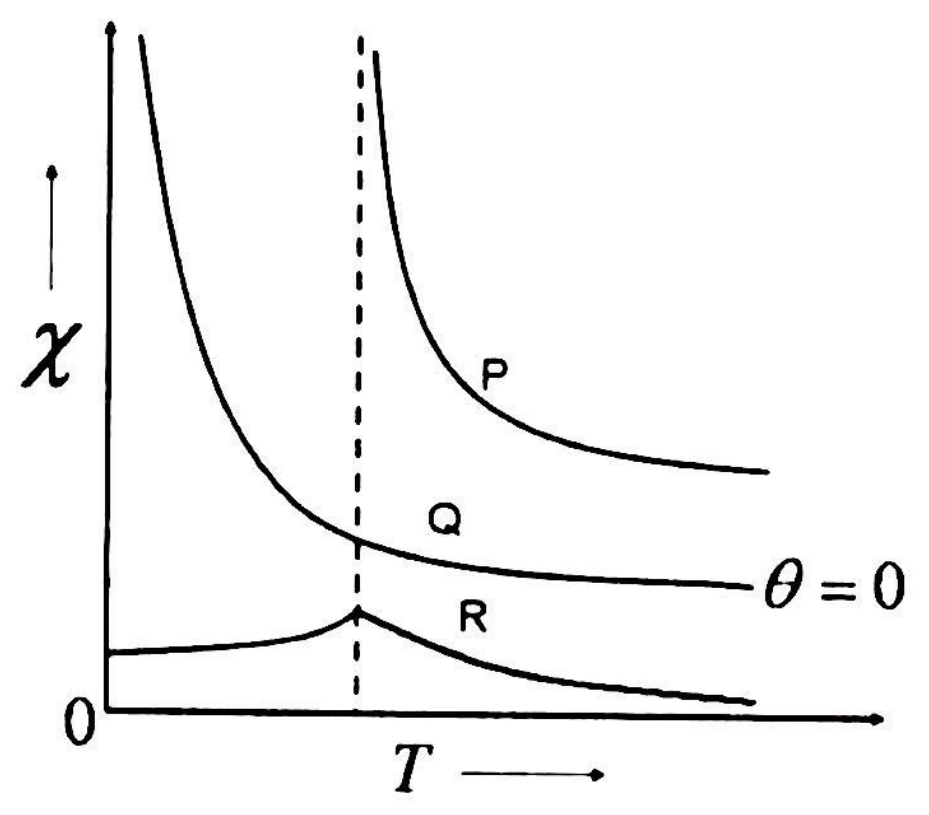
\includegraphics[width=2.5cm]{figs/Q27.png}
    \end{figure}
    \newpage
     Which of the following statements is correct?
    \begin{enumerate}
   	\item Curve R represents a paramagnet and Q a ferromagnet
   	\item Curve Q represents a ferromagnet and P an antiferromagnet
   	\item Curve R represent an antiferromagnet and Q a paramagnet
   	\item Curve R represents an antiferromagnet and Q a ferromagnet
   \end{enumerate}
   
%28
    \item The dielectric constant of a material at optical frequencies is mainly due to 
    \begin{enumerate}
    	\item ionic polarizability
    	\item electronic polarizability
    	\item dipolar polarizability
    	\item ionic and dipolar polarizability
    \end{enumerate}
%29
    \item An electron of wavevector $\vec{k_e}$, velocity $\vec{v_h}$, and effective mass $m_h$. Which one of the following statements is correct?
    \begin{enumerate}
    	\item $\vec{k_h}=-\vec{k_e};\vec{v_h}=-\vec{v_e};m_h=-m_e$
    	\item $\vec{k_h}=\vec{k_e};\vec{v_h}=\vec{v_e};m_h=m_e$
    	\item $\vec{k_h}=\vec{k_e};\vec{v_h}=-\vec{v_e};m_h=-m_e$
    	\item $\vec{k_h}=-\vec{k_e};\vec{v_h}=\vec{v_e};m_h=-m_e$
   \end{enumerate}
%30 
    \item In a diatomic molecule, the internuclear separation of the ground and first excited electronic state are the same as shown in the figure.
    \begin{figure}[!ht]
    \centering
    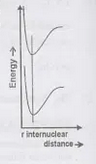
\includegraphics[width=2cm]{figs/Q30.png}
    \caption{}
    \end{figure}
    \newpage
     If the molecule is initially in the lowest vibrational state of the ground state, then the absorption spectrum will appear as
\begin{enumerate}
\item \begin{figure}[!ht]
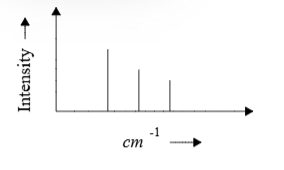
\includegraphics[width=2.5cm]{figs/optionA.png}
\end{figure}
\item \begin{figure}[!ht]
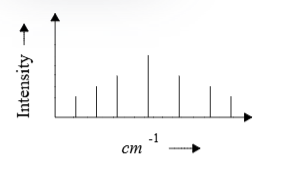
\includegraphics[width=2.5cm]{figs/optionB.png}
\end{figure}
\item \begin{figure}[!ht]
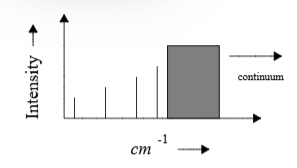
\includegraphics[width=2.5cm]{figs/optionC.png}
\end{figure}
\item \begin{figure}[!ht]
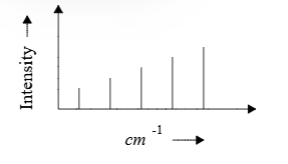
\includegraphics[width=2.5cm]{figs/optionD.png}
\end{figure}
\end{enumerate}
%31
    \item Five energy levels of a system including the ground state are shown below. Their lifetimes and the allowed electric dipole transitions are also marked.\\
    \begin{figure}[!ht]
\centering
\resizebox{0.5\textwidth}{!}{%
\begin{circuitikz}
\tikzstyle{every node}=[font=\large]


\draw (5.75,16.5) to[short] (15.5,16.5); 
\draw (5.75,14.5) to[short] (15.5,14.5); 
\draw (5.75,12.75) to[short] (15.5,12.75); 
\draw (5.75,11) to[short] (15.5,11);     
\draw (5.75,9.25) to[short] (15.5,9.25); 


\draw [->, >=Stealth] (7.75,16.5) -- (7.75,14.5);
\draw [->, >=Stealth] (9.75,16.5) -- (9.75,12.75);
\draw [->, >=Stealth] (12,14.5) -- (12,9.25);
\draw [->, >=Stealth] (14,11) -- (14,9.25);
\draw [->, >=Stealth] (6.75,12.75) -- (6.75,9.25);


\node[anchor=west] at (15.5,16.5) {4};
\node[anchor=west] at (15.5,14.5) {3};
\node[anchor=west] at (15.5,12.75) {2};
\node[anchor=west] at (15.5,11) {1};
\node[anchor=west] at (15.5,9.25) {0};


\node[anchor=south] at (10.5,16.5) {$10^{-7}$ s};
\node[anchor=south] at (10.5,14.5) {$2 \times 10^{-8}$ s};
\node[anchor=south] at (10.5,12.75) {$10^{-6}$ s};
\node[anchor=south] at (10.5,11) {$10^{-8}$ s};

\end{circuitikz}
}%
\end{figure}\\
    Which one of the following transitions is the most suitable for a continuous wave \brak{CW} laser?
    \begin{enumerate}
    	\item $1\rightarrow 0$
    	\item $2\rightarrow 0$
    	\item $4\rightarrow 2$
    	\item $4\rightarrow 3$
    \end{enumerate}  
%32
    \item Assuming the mean life time of a muon \brak{\text{in its rest frame}} to be $2\times 10^{-6}s$, its life time in the laboratory frame, when it is moving with a velocity $0.95c$ is 
    \begin{enumerate}
    	\item $6.4\times 10^{-6}s$
    	\item $0.62\times 10^{-6}s$
    	\item $2.16\times 10^{-6}s$
    	\item $0.19\times 10^{-6}s$
    \end{enumerate}
%33
    \item Cesium has a nuclear spin of $7/2$. The hyperfine spectrum of the D lines of the cesium atom will consist of
    \begin{enumerate}
        \item 10 lines
        \item 4 lines
        \item 6 lines
        \item 14 lines
    \end{enumerate}
%34 
    \item The probability that an energy level $\varepsilon$ at a temperature $T$ is \textit{unoccupied} by a fermion of chemical potential $\mu$ is given by
    \begin{enumerate}
        \item $\frac{1}{e^{\brak{\varepsilon - \mu} / k_B T} + 1}$
        \item $\frac{1}{e^{\brak{\varepsilon - \mu} / k_B T} - 1}$
        \item $\frac{1}{e^{\brak{\mu - \varepsilon} / k_B T} + 1}$
        \item $\frac{1}{e^{\brak{\mu - \varepsilon} / k_B T} - 1}$
    \end{enumerate}
%35 
    \item Consider the following expression for the mass of a nucleus with $Z$ protons and $A$ nucleons:\\
    $
    M\brak{A, Z} = \frac{1}{c^2} \brak{f\brak{A} + yZ + zZ^2}
    $
    Here, $f\brak{A}$ is a function of $A$,
    \begin{align*}
    y = -4a_A, \quad z = a_c A^{-1/3} + 4a_A A^{-1}
    \end{align*}
    $a_A$ and $a_c$ are constants of suitable dimensions. For a fixed $A$, the expression of $Z$ for the most stable nucleus is
    \begin{enumerate}
        \item $Z = \frac{A / 2}{1 + \brak{\frac{a_c}{a_A}} A^{2/3}}$
        \item $Z = \frac{A / 2}{1 + \brak{\frac{a_c}{4a_A}} A^{2/3}}$
        \item $Z = \frac{A}{1 + \brak{\frac{a_c}{4a_A}} A^{2/3}}$
        \item $Z = \frac{A}{1 + A^{2/3}}$
    \end{enumerate}
%36 
    \item The de Broglie wavelength of particles of mass $m$ with average momentum $p$ at a temperature $T$ in three dimensions is given by
    \begin{enumerate}
        \item $\lambda = \frac{h}{\sqrt{2mk_B T}}$
        \item $\lambda = \frac{h}{\sqrt{3mk_B T}}$
        \item $\lambda = \frac{h}{\sqrt{2k_B T}}$
        \item $\lambda = \frac{h}{\sqrt{3m}}$
    \end{enumerate}
\end{enumerate}
\end{document}

